\documentclass{beamer}
\usepackage{config}

%Information to be included in the title page:
\title[Git seul connecté mono-branche]{Git : mode d'emploi pour un usage seul, avec dépôt distant, sur une seule branche}
\author{Florian Legendre}
\institute{Université de Poitiers}
\date{Année 2020 - 2021}
\logo{
\includegraphics[scale=0.1]{UP.png}}


%%% ============================================================= %%%
%%% ====================== Début des diapos ===================== %%%
%%% ============================================================= %%%

\begin{document}

\frame{\titlepage}

\begin{frame}
\frametitle{Table of Contents}
\tableofcontents[hideallsubsections]
\end{frame}


%% --------------------- %%
%%        SECTION        %%
%% --------------------- %%
\AtBeginSection[]
{
  \begin{frame}
    \frametitle{Table of Contents}
    \tableofcontents[sectionstyle=show/hide,subsectionstyle=show/show/hide]
  \end{frame}
}
\section{Configurer le suivi d'une branche distante}

% Subsection:
\subsection{Cloner un projet}

\begin{frame}[fragile]
\frametitle{Commande: git clone <url>}
\begin{mdframed}[style=Bash]
    \begin{lstlisting}[style=Bash, caption={Exemple de git clone}]
crex@crex:~/projects$ git clone https://github.com/torvalds/linux.git
Cloning into 'linux'...
remote: Enumerating objects: 7886755, done.
remote: Total 7886755 (delta 0), reused 0 (delta 0), pack-reused 7886755
Receiving objects: 100% (7886755/7886755), 2.98 GiB | 1.12 MiB/s, done.
Resolving deltas: 100% (6548657/6548657), done.
Updating files: 100% (71277/71277), done.
    \end{lstlisting}
    \end{mdframed}
\end{frame}

\subsection{Suivre une branche distante}
\begin{frame}
\frametitle{Commandes: git remote add <al> <url> / git remote rm <al>}
La première commande "git remote add" suivi d'un alias et d'une url permettent de suivre la branche distante désignée par l'url.\\
\smallskip

Un alias est un comme un pseudo donné à l'url il permet:
\begin{enumerate}
    \item De spécifier où faire le push d'une branche:\\ git push <al> <nomBrancheDistante>
    \item De spécifier quelle branche du dépôt distant on veut pull:\\ git pull <al> <nomBrancheDistante>
    \item De supprimer un suivi de branche distante:\\ git remote rm <al>
    \item De spécifier une branche où on veut push/pull par défaut:\\ git push $--$set-upstream <al> <nomBrancheDistante>
\end{enumerate}
\end{frame}

\begin{frame}[fragile]{Commande: git remote -v}
Comme pour les branches locales on peut vouloir savoir quelle branche distante on suit actuellement ou encore l'ensemble des alias vers des url que contient notre branche locale. Ces informations sont accessibles par la commande \textit{git remote -v}.
\medskip

Exemple:
\begin{mdframed}[style=Bash]
\begin{lstlisting}[style=Bash, caption=Exemple d'output de la commande git remote -v]
crex@crex:~/projects/GitLearn(main)$ git remote -v
origin	git@github.com:Chuxclub/GitLearn.git (fetch)
origin	git@github.com:Chuxclub/GitLearn.git (push)
\end{lstlisting}
\end{mdframed}

\end{frame}



%% --------------------- %%
%%        SECTION        %%
%% --------------------- %%
\AtBeginSection[]
{
  \begin{frame}
    \frametitle{Table of Contents}
    \tableofcontents[sectionstyle=show/hide,subsectionstyle=show/show/hide]
  \end{frame}
}
\section{Synchroniser son travail}

% Subsection:
\subsection{Récupérer les modifications d'un serveur distant}
\begin{frame}
\frametitle{Commandes: git fetch / git pull}

\begin{tabular}{ | m{13em} | m{13em} | }
    \hline
    
    \textbf{git fetch} & \textbf{git pull}\\
        
    \hline
    
    \begin{enumerate}
        \item Récupère seulement la dernière mise à jour de l'historique
        \item Il faut ensuite faire un git merge pour incorporer les changements
        \item Utile quand on veut anticiper des conflits ou qu'on n'a pas tout à fait fini son travail
    \end{enumerate}
    & 
    
    \begin{enumerate}
    \item Récupère seulement la dernière mise à jour de l'historique et incorpore les changements simultanément
    \item Elle est plus utilisée que git fetch
    \end{enumerate} \\
    
    \hline
\end{tabular}

\end{frame}


% Subsection:
\subsection{Ajouter ses mises à jour sur un serveur distant}
\begin{frame}
\frametitle{Commande: git push}
La commande "git push" permet de mettre à jour la branche distante en incorporant dans la branche distante l'historique et les fichiers locaux.
\bigskip

\textbf{ATTENTION:} 
\begin{enumerate}
    \item Il faut avoir fait un git pull avant de l'utiliser
    \item Il faut avoir les droits
\end{enumerate}
\end{frame}


%% --------------------- %%
%%        SECTION        %%
%% --------------------- %%
\AtBeginSection[]
{
  \begin{frame}
    \frametitle{Table of Contents}
    \tableofcontents[sectionstyle=show/hide,subsectionstyle=show/show/hide]
  \end{frame}
}
\section{La boucle de travail multibranches connectées}

\begin{frame}{La boucle de travail multibranches connectées}
\begin{center}
	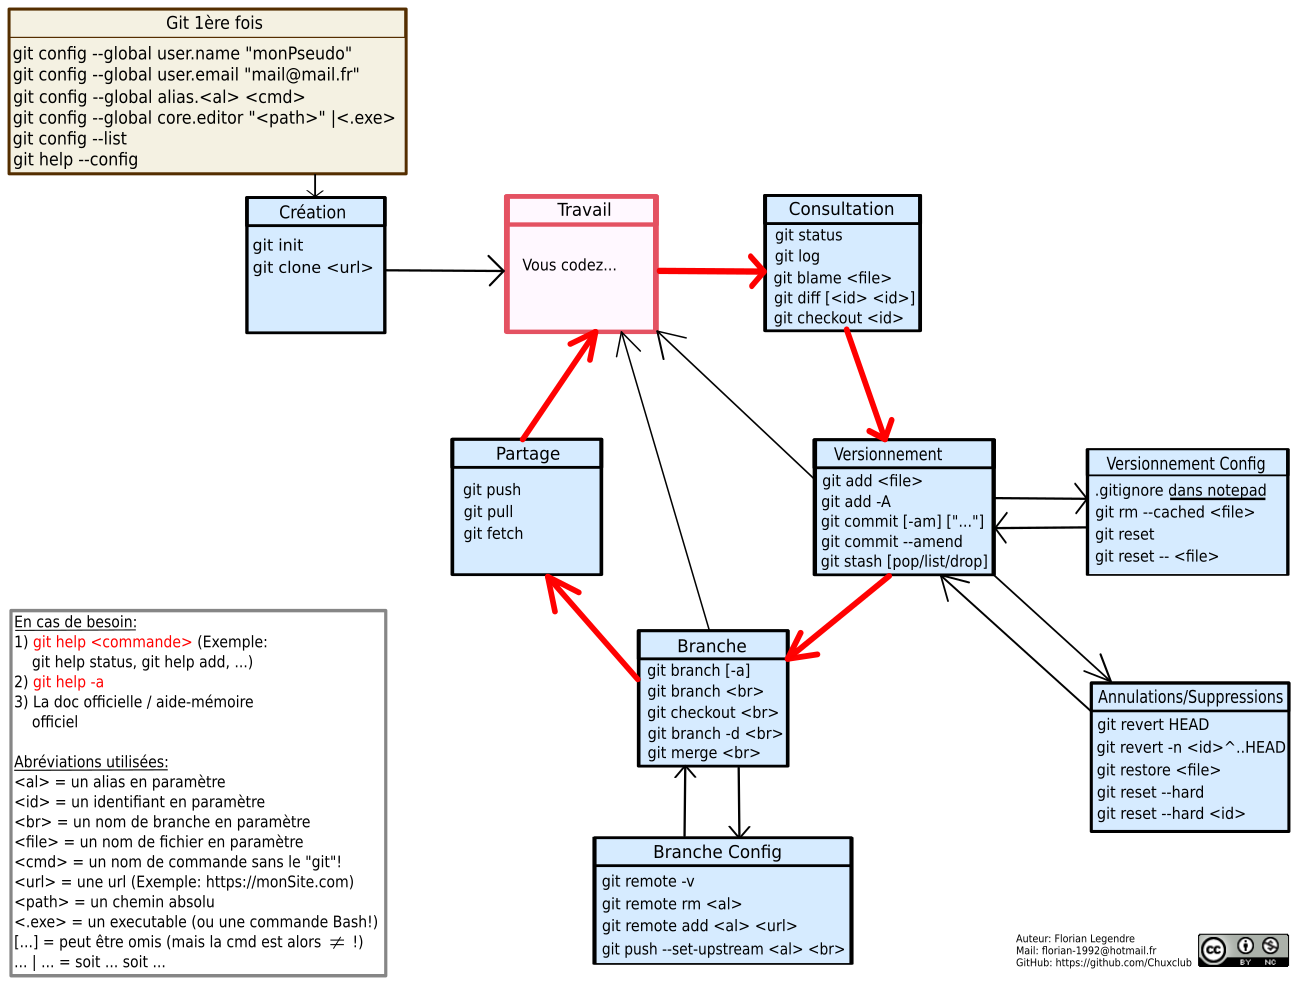
\includegraphics[scale=0.3]{gitCommandFlow/gitCommandFlow_connectedLoop.png}
\end{center}
\end{frame}


\end{document}